\chapter{SUBMITTER CONTRIBUTION}

\section{Submitter Role in the RollupX Pipeline}

The Submitter is the component responsible for connecting the off-chain rollup execution pipeline with the Layer-1 settlement environment. In the RollupX prototype, earlier pipeline stages such as the Sequencer, Executor, and Prover prepare a finalized batch containing transaction data, state transition metadata, proof metadata, and the resulting state root. The Submitter receives this finalized batch information and converts it into a Layer-1 submission according to the configured data availability strategy.

The internal flow executes as follows: Finalized batch input $\rightarrow$ DA strategy selection $\rightarrow$ DA payload encoding $\rightarrow$ \texttt{BridgeClient::commit\_batch} $\rightarrow$ L1 transaction hash $\rightarrow$ receipt polling/confirmation $\rightarrow$ receipt-status validation $\rightarrow$ metrics/export.

Figure \ref{fig:submitter_pipeline} illustrates the internal pipeline and settlement flow of the Submitter service, identifying the sequence from batch retrieval to final L1 settlement metrics export. This figure is reused from the final project report.

\begin{figure}[htbp]
\centering
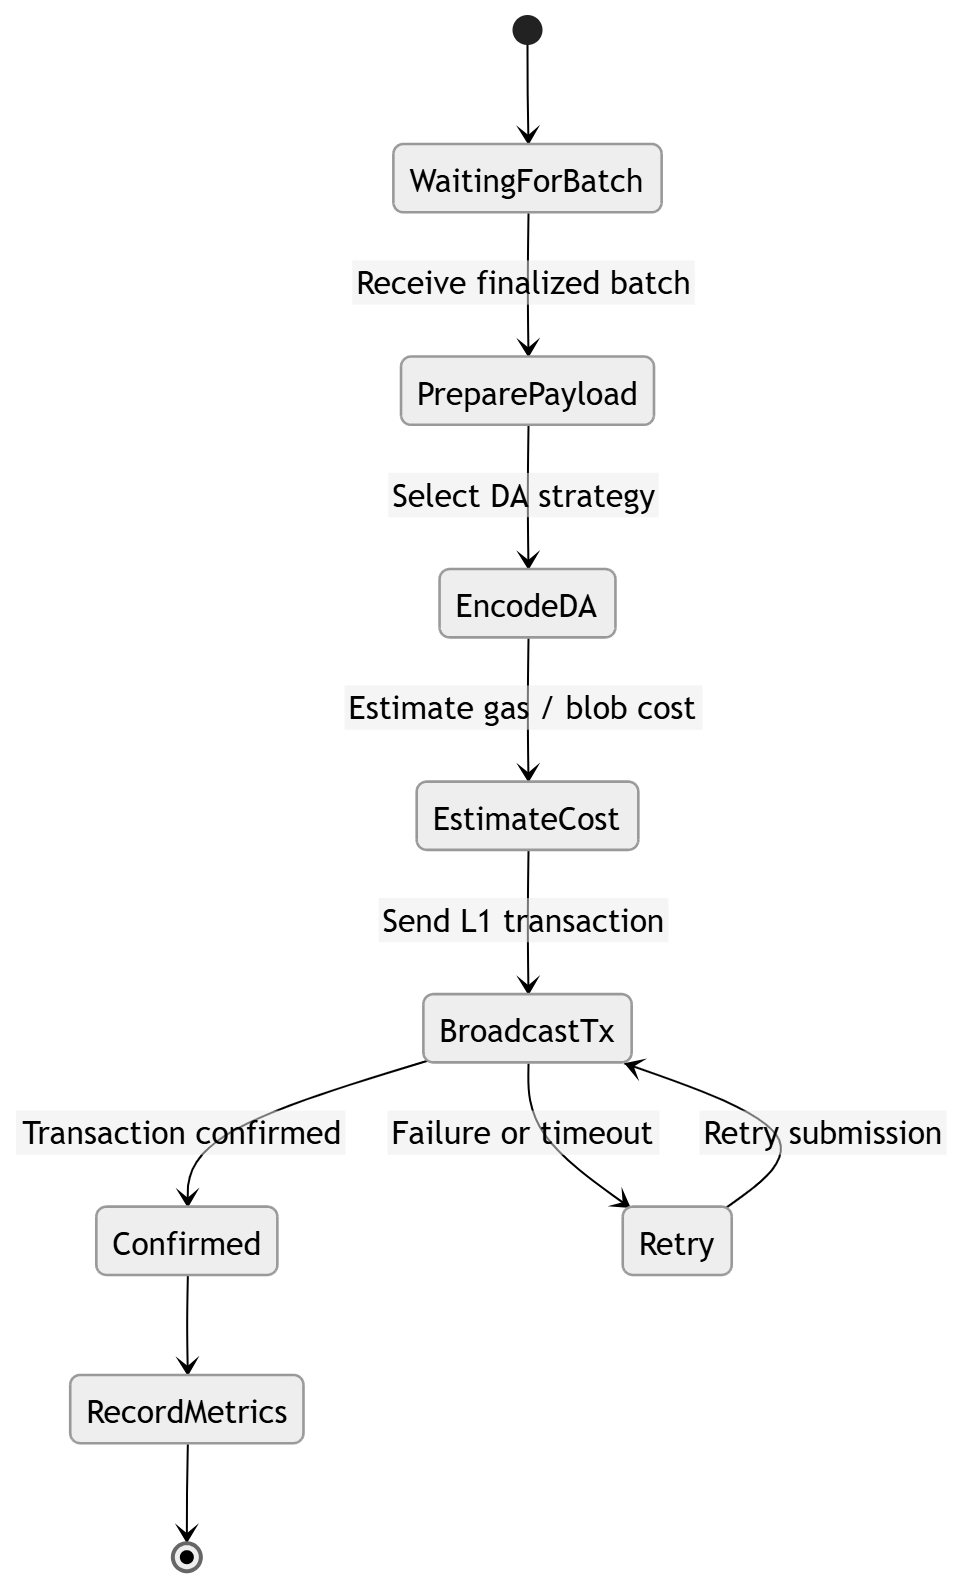
\includegraphics[width=0.8\textwidth]{../final_report/figures/chapter5/submitter_settlement_flow.png}
\caption{Submitter settlement flow diagram (reused from final report), showing the sequence of operations from batch retrieval to metrics export across my implementation modules.}
\label{fig:submitter_pipeline}
\end{figure}

At a code level, the Submitter performs four main responsibilities, as summarized below:
\begin{table}[!htbp]

\centering
\caption{Submitter Internal Pipeline Steps}
\label{tab:submitter_internal_flow}
\small
\setlength{\tabcolsep}{3pt}
\renewcommand{\arraystretch}{1.15}
\begin{tabularx}{\textwidth}{|
>{\raggedright\arraybackslash}p{0.13\textwidth}|
>{\raggedright\arraybackslash}p{0.23\textwidth}|
>{\raggedright\arraybackslash}p{0.15\textwidth}|
>{\raggedright\arraybackslash}X|
>{\raggedright\arraybackslash}p{0.14\textwidth}|}
\hline
\textbf{Step} & \textbf{Code Location} & \textbf{Input} & \textbf{Processing} & \textbf{Output} \\ \hline

Batch Poll &
\path{storage_postgres.rs} &
Batch ID &
Fetches pending batch records from the storage layer. &
\texttt{Batch} struct \\ \hline

Encoding &
\path{da_blob.rs}, \path{da_calldata.rs} &
\texttt{Batch} &
Encodes the batch according to the selected data availability strategy and prepares DA metadata. &
DA payload \\ \hline

Submission &
\path{ethereum_adapter.rs} &
Payload and proof metadata &
Calls the L1 bridge contract method through the Ethereum adapter. &
Transaction hash \\ \hline

Verification &
\path{ethereum_adapter.rs} &
Transaction hash &
Polls the L1 transaction receipt and checks whether \texttt{status == 1}. &
Confirmation result \\ \hline

\end{tabularx}
\end{table}



This component was important to the project because it formed the boundary between the local Layer-2 benchmark pipeline and the Layer-1 contract environment. Without a working Submitter, the benchmark framework could measure only internal L2 processing. With the Submitter, the system could also evaluate settlement latency, Layer-1 submission cost, data availability footprint, and the reliability of different DA configurations.

\section{Submitter Architecture and Refactor}

My main Submitter contribution was the refactoring and organization of the Submitter service into a cleaner application structure. Commit \texttt{e4dad07} provides the main evidence for this work. The refactor removed duplicate or legacy entry-point logic from files such as \path{src/main.rs} and \path{src/submitter.rs}, and centralized the submission workflow inside the application-level orchestrator.

The orchestrator, located in \path{submitter/src/application/orchestrator.rs}, acts as the control layer of the Submitter. Its role is not to directly encode every DA format or directly interact with Ethereum RPC calls. Instead, it coordinates the submission lifecycle by selecting the configured strategy, passing finalized batch data into that strategy, handling the returned transaction hash or receipt result, and ensuring that the final status is visible to the metrics and logging layers.

This separation improved the maintainability of the Submitter because the high-level submission workflow was separated from low-level infrastructure concerns. The application layer could describe \textit{what} should happen during a batch submission, while infrastructure modules such as the Ethereum adapter and DA strategy files implemented \textit{how} that submission is performed.

\section{Code-Level Abstraction: The \texttt{BridgeClient} Trait}

A key part of the Submitter refactor was the introduction of the \texttt{BridgeClient} abstraction in \path{submitter/src/infrastructure/ethereum_adapter.rs}. The purpose of this trait was to decouple the Submitter and DA strategy code from a concrete Ethereum client implementation such as \texttt{ethers::Provider}. Instead of allowing each DA strategy to directly create provider calls and contract bindings, the DA modules communicate through a common bridge interface.

Exact excerpt from \path{submitter/src/infrastructure/ethereum\_adapter.rs}:

\newpage
\begin{lstlisting}[language=C, numbers=left, breaklines=true, basicstyle=\ttfamily\small]
#[async_trait]
pub trait BridgeClient: BridgeReader + Send + Sync {
    async fn commit_batch(
        &self,
        da_id: u8,
        verifier_id: u8,
        batch_data: Bytes,
        da_meta: Bytes,
        new_root: [u8; 32],
        proof: Bytes,
    ) -> Result<H256, DomainError>;
}
\end{lstlisting}

The input to this interface is the finalized batch submission data: the data availability mode identifier, verifier identifier, encoded batch data, DA metadata, new state root, and proof bytes (which may contain a mock verifier representation or real Groth16 bytes). The output is either a Layer-1 transaction hash or a domain-level error. This allowed the Submitter to treat different Layer-1 submission paths consistently while keeping Ethereum-specific implementation details inside the infrastructure layer.

The technical value of this change was testability. By programming against the \texttt{BridgeClient} trait, the DA strategy code and orchestrator logic could be tested using mock bridge clients instead of requiring a live Hardhat or Anvil network for every unit test. This made it possible to simulate successful submissions, reverted transactions, delayed confirmations, and error paths in a controlled way.

\section{Data Availability Strategy Implementations}

The Submitter supports multiple data availability strategies so that the benchmark suite can compare different L1 data publication models under a consistent pipeline. Figure \ref{fig:da_strategies} illustrates the three supported data publication paths. This final-report figure is reused to show the architectural impact of the DA module code I contributed.

\begin{figure}[htbp]
\centering
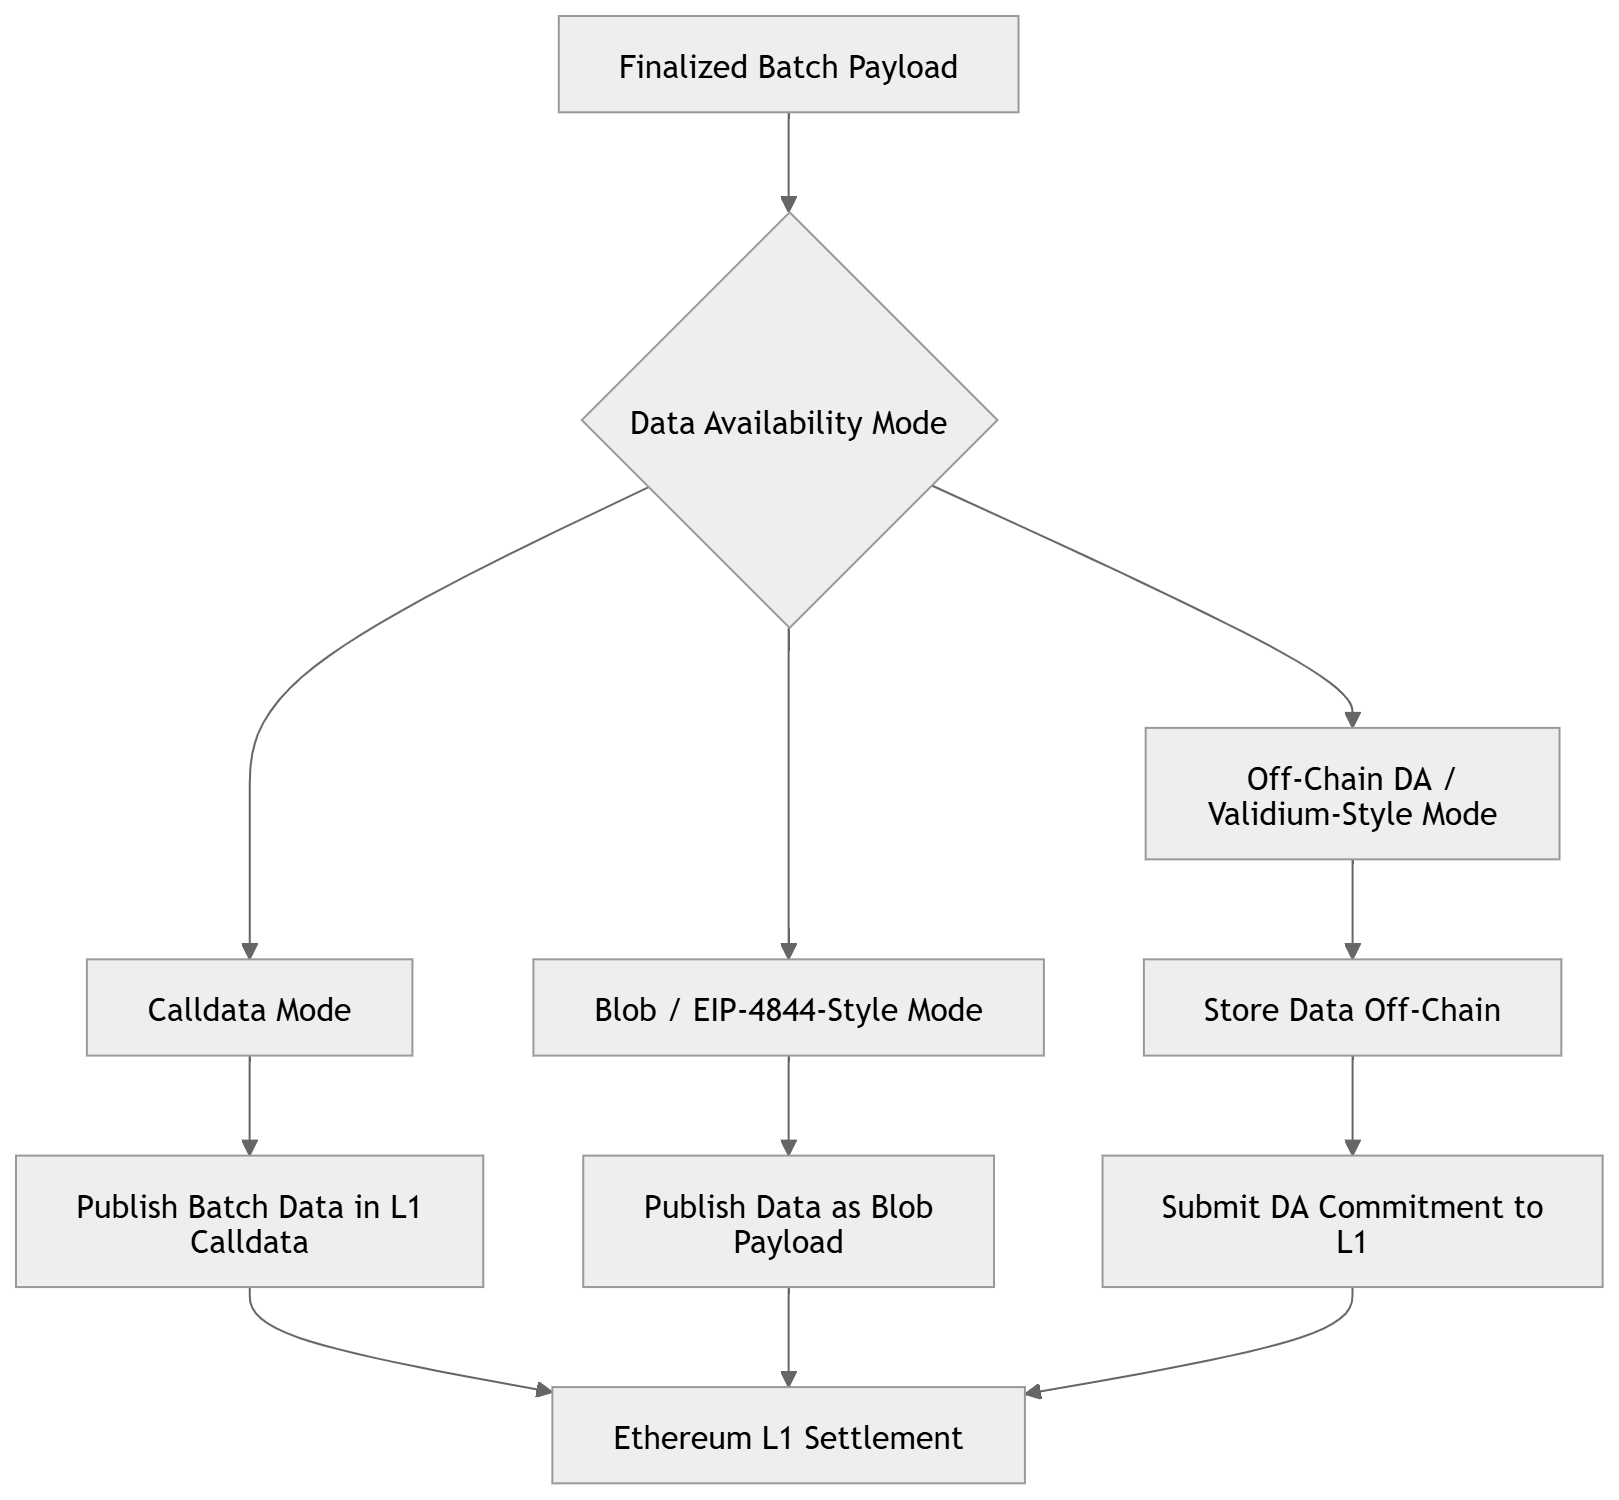
\includegraphics[width=\textwidth]{../final_report/figures/chapter3/da_com.png}
\caption{Data Availability strategy diagram (reused from final report) showing the three available benchmark paths: Calldata, Blob-style, and Off-chain.}
\label{fig:da_strategies}
\end{figure}

My contribution included implementing and refactoring the concrete DA strategy modules used by the Submitter, summarized in Table \ref{tab:da_strategies}.

\begin{table}[!htbp]
\centering
\caption{Data Availability Strategy Comparison}
\label{tab:da_strategies}
\small
\setlength{\tabcolsep}{3pt}
\renewcommand{\arraystretch}{1.15}
\begin{tabularx}{\textwidth}{|
>{\raggedright\arraybackslash}p{0.15\textwidth}|
>{\raggedright\arraybackslash}p{0.19\textwidth}|
>{\raggedright\arraybackslash}p{0.12\textwidth}|
>{\raggedright\arraybackslash}X|
>{\raggedright\arraybackslash}p{0.22\textwidth}|}
\hline
\textbf{DA Strategy} &
\textbf{File} &
\textbf{Input} &
\textbf{L1 Payload / Metadata} &
\textbf{Benchmark Purpose} \\ \hline

Calldata &
\path{da_calldata.rs} &
\texttt{Batch} &
Encodes batch data directly into the L1 submission payload. The DA metadata field is empty or minimal depending on the submission path. &
Provides the baseline L1 data-publication cost and latency measurement. \\ \hline

Blob-style &
\path{da_blob.rs} &
\texttt{Batch} &
Prepares blob-style DA metadata or commitment information for the benchmark-mode blob path. &
Evaluates the cost and footprint impact of an EIP-4844-style DA configuration. As detailed in the final report, this mode achieved an approximately 70\% cost reduction over Calldata DA. \\ \hline

Off-chain &
\path{da_offchain.rs} &
\texttt{Batch} &
Keeps batch data outside L1 and submits off-chain pointer or commitment-style metadata. &
Models a Validium-style low-L1-data configuration for comparison, achieving an 82.5\% cost reduction. \\ \hline

\end{tabularx}
\end{table}


\subsection{Calldata Data Availability}

The calldata data availability path is implemented in \path{submitter/src/infrastructure/da_calldata.rs}. This strategy prepares the finalized batch payload for submission as Layer-1 calldata. In this mode, the batch data or encoded batch representation is included directly in the transaction payload passed to the bridge contract.

The main input to this module is the finalized batch data received from the orchestrator. The strategy encodes this data into the format expected by the \texttt{BridgeClient::commit\_batch} interface, attaches the relevant DA metadata, and submits the resulting payload through the Ethereum adapter. Its output is the transaction hash and, after confirmation, the receipt-derived status used by the Submitter metrics layer.

This mode is important for benchmarking because calldata is the traditional data publication method used by many rollup designs. Measuring calldata submission gives a baseline for comparing newer or alternative DA strategies.

\subsection{Blob-Style Data Availability}

The blob-style data availability path is implemented in \path{submitter/src/infrastructure/da_blob.rs}. In the RollupX benchmark environment, this mode represents an EIP-4844-style data availability configuration. The purpose of this module is to separate blob-style batch publication logic from calldata publication logic so that the benchmark suite can compare the cost and footprint of different DA configurations.

This module prepares blob-mode payload metadata and submits the corresponding commitment information through the same bridge abstraction used by the calldata strategy. Depending on the local benchmark environment, the blob-mode implementation may model blob-style submission behaviour rather than providing the full production Ethereum blob transaction path. Therefore, this report describes it as an EIP-4844-style benchmark mode rather than a production blob submission implementation.

\subsection{Off-Chain Data Availability}

The off-chain data availability path is implemented in \path{submitter/src/infrastructure/da_offchain.rs}, where present in the repository history. This mode supports a validium-style benchmark configuration in which the full batch data is not posted directly to Layer 1. Instead, the Submitter records or references the payload off-chain and submits only commitment-style metadata to the L1 bridge contract.

This mode was useful for the research framework because it provided a low-L1-data-cost configuration for comparison against calldata and blob-style modes. However, it should be interpreted as a local research stub for studying cost and performance trade-offs, not as a production validium data availability system.

\section{L1 Submission, Receipt Handling, and Metrics}

The Submitter submission lifecycle does not end when a transaction hash is produced. A transaction hash only indicates that the transaction was broadcast or accepted by the local client. For benchmark correctness, the Submitter must wait until the transaction is mined and then inspect the receipt to determine whether the L1 execution actually succeeded.

My contribution included the infrastructure required to support this lifecycle. The persistence and state-handling modules, such as \path{submitter/src/infrastructure/storage_postgres.rs} and \path{submitter/src/infrastructure/storage_sqlite.rs}, support storing submission state and benchmark-related records. The observability module, \path{submitter/src/infrastructure/observability.rs}, exposes submission metrics so that the benchmark pipeline can later analyse the L1 submission stage together with Sequencer, Executor, and Prover metrics.

The main metrics produced by the Submitter are related to settlement behaviour: submission latency, confirmation time, transaction success or failure, gas usage where available, and data availability mode metadata. These metrics are later consumed by the data-tools pipeline to compute final experimental summaries such as cost per transaction, finalization time, and DA footprint.

\section{Submitter Bug Fix: Silent L1 Revert Detection}

One of the most important reliability fixes in the Submitter was the correction of silent Layer-1 transaction revert handling. Before this fix, the Submitter could treat a mined transaction as successful even if the EVM execution reverted. This is a subtle but serious problem because a transaction can be included in a block while still failing at the smart contract execution layer.

In commit \texttt{e4dad07}, I added explicit receipt-status validation in both \path{submitter/src/infrastructure/da_calldata.rs} and \path{submitter/src/infrastructure/da_blob.rs}. The key logic checks the receipt status field and treats only status value \texttt{1} as a successful L1 execution.

Exact excerpt from \path{submitter/src/infrastructure/da_blob.rs} (similar logic exists in \texttt{da_calldata.rs}):

\begin{lstlisting}[language=C, numbers=left, breaklines=true, basicstyle=\ttfamily\small]
if let Some(status) = r.status {
    if status.as_u64() == 1 {
        // success path
    } else {
        warn!("Tx {} reverted!", tx_hash);
        return Err(DomainError::Da(
            "Transaction reverted on-chain".to_string()
        ));
    }
}
\end{lstlisting}

The root cause of the issue was the difference between transaction mining and transaction success. A mined transaction only confirms that the transaction reached the chain. It does not guarantee that the called contract function executed successfully. Without checking the receipt status, the Submitter could record a failed bridge submission as a successful benchmark result.

The fix improved experimental correctness. If an L1 bridge call failed due to out-of-gas, invalid calldata, contract validation failure, or other EVM-level errors, the Submitter would now return a domain error instead of silently treating the result as successful. This prevented incorrect success counts, inaccurate finalization measurements, and misleading cost or latency results.

\section{Submitter Testing, Mocking, and Coverage}

The introduction of the \texttt{BridgeClient} abstraction also improved the testability of the Submitter. The tests in \path{submitter/tests/integration_test.rs} could use mock bridge behaviour to validate the Submitter workflow without depending on a live Layer-1 node for every test case. This made it possible to test success paths, failed confirmations, revert handling, and strategy-level behaviour more reliably.

Commit \texttt{e4dad07} also added CI and coverage-related workflow support, including files such as \path{submitter/.github/workflows/coverage.yml} and \path{submitter/.github/workflows/ci.yml}. These workflows used Rust testing and coverage tooling such as \texttt{tarpaulin} to make Submitter quality measurable. The contribution evidence records an increase in verifiable Submitter test coverage from approximately 41\% to 88\%, which reflects the impact of the refactor and mock-based testing structure.

Overall, the Submitter contribution added the L1 settlement path required by RollupX, introduced a testable architecture around the \texttt{BridgeClient} abstraction, implemented multiple data availability submission modes, improved receipt-level reliability, and exposed metrics required for end-to-end benchmark analysis.

